
\chapter{Methodology}
\begin{refsection}
% text of this chapter goes here

 This chapter explains the methods used to develop the Helmet Compliance Detection Using Computer Vision. It includes data collection, prototypes development using the YOLO algorithm, integration of added features, and testing to ensure the prototype performs well in real-time detection of traffic violations.

\section*{Research Design}
 
 Constructive research design involves the development of new prototypes or solutions based on existing knowledge and theories. This methodology enables researchers to create practical, functional solutions that can be implemented in real-world scenarios. It focuses on addressing real-world challenges by combining theoretical insights with practical applications. In fields such as technology and computer science, constructive research typically involves the creation of software or systems that enhance or refine existing solutions, all while building on established principles to improve functionality and effectiveness \cite{Lassenius2001}.

This study will use a constructive research design to develop a real-time helmet compliance detection prototype that enhances road safety monitoring through the use of AI powered technologies. This research design is appropriate for the study because it focuses on building a functional and innovative prototype that integrates computer vision compo
nents to address the identified gaps in traffic law enforcement. This study will develop an intelligent detection prototype that is capable of identifying motorcycle riders without helmets, improper helmet usage, overloading of passengers, and missing or unreadable license plates. The protoype will use the YOLOv8 object detection algorithm for real-time identification, OpenCV for visual processing. It will also trigger alerts and automatically record  violations for documentation and enforcement purposes. The prototype is designed for use along Nabua Highway,Camarines Sur, the prototype aims to function effectively even in varying lighting and weather conditions. By constructing and evaluating this prototype, the study contributes a practical and scalable solution to improve road safety compliance using modern AI techniques. Adopting constructive research allows this study to develop a practical solution for improving road safety. In everyday life, many accidents happen because riders don’t wear helmets. To address this issue, this study will build a prototype that automatically checks if riders are wearing helmets using computer vision. The prototype will use a detection algorithm to identify helmets in real-time. Through testing and collecting more data, the prototype will be improved to make it more accurate. The goal is to build a prototype that traffic authorities can use to check helmet compliance and improve road safety. This study will help to make the roads safer and can help prevent accidents and save lives.




\section*{ Theorems, Algorithm and Mathematical Framework}


In the field of computer vision, algorithms and mathematical models are important in developing systems e for real-time object detection. This study uses a YOLOv8-based approach to detect helmet usage, count motorcycle passengers, and recognize license plates. YOLO (You Only Look Once) is a single-stage object detection algorithm known for its speed and
accuracy, making it suitable for deployment in real-time environments.


\section*{ YOLOv8 Object Detection Algorithm}


YOLOv8 is the latest version of the YOLO family of algorithms, designed for fast and accurate object detection. Unlike previous versions, YOLOv8 introduces an anchor-free architecture, improved feature extraction, and decoupled detection heads for classification and localization, making it more flexible and precise. According to \citeauthor{Muhammad2024} [\citeyear{Muhammad2024}] YOLOv8 was used for real-time helmet detection in Indonesia, achieving a 91.1\% F1 score for helmet detection and 81.7 \% accuracy for rider detection \cite{Muhammad2024}. This study highlights YOLOv8's effectiveness in real-world applications, emphasizing its potential for smart city integration and law enforcement, particularly in monitoring motorcyclist safety.

YOLOv8 works by predicting bounding boxes and class probabilities directly from full images in one evaluation, treating detection as a regression problem. As illustrated in Figure 1, the algorithm follows a streamlined architecture composed of an input layer, backbone, neck, and prediction head, resulting in accurate and real-time object detection. It employs advanced loss functions, such as Complete Intersection over Union (CIoU), to improve bounding box accuracy. The algorithm also utilizes Non-Maximum Suppression (NMS), which filters overlapping bounding boxes and retains only the most confident predictions. Furthermore, YOLOv8 outputs are detected only when the confidence score exceeds a predefined threshold, reducing false positives.

\begin{figure}[H]
    \centering
    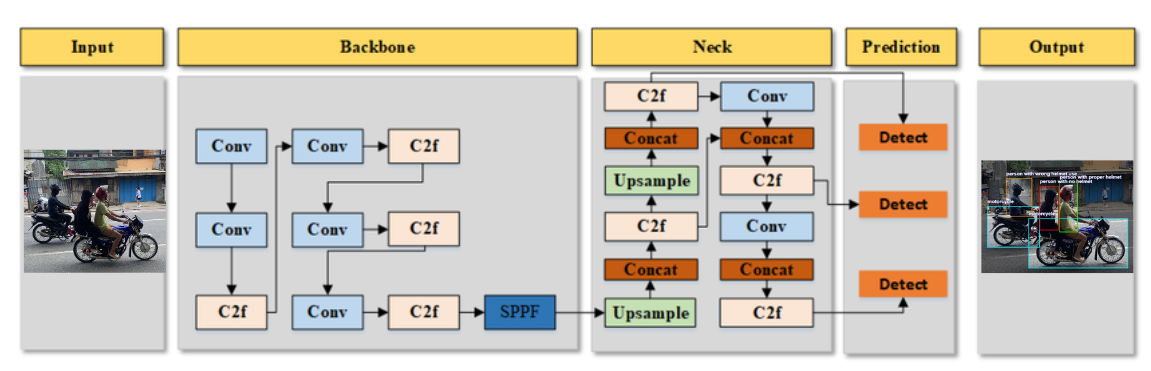
\includegraphics[width=1\textwidth]{figures/Fig 1.png} % 75% of text width
    \caption{\textbf{Yolov8 Object Detection Architecture}}
    \label{fig:yolov8_architecture}
\end{figure}




Figure 1 illustrates the YOLOv8 architecture, where the input image is first resized  and normalized, then passed through the backbone for feature extraction using convolutional layers  and C2f blocks, followed by the neck that refines and fuses multi-scale features through concatenation  and upsampling, and finally through a decoupled prediction head for separate classification and  localization, producing bounding boxes and labels.




\section*{Detection Mechanism of Yolov8}


\subsection*{Bounding Box Prediction}


YOLOv8 predicts the center coordinates $(x_{pred}, y_{pred})$, width $(w_{pred})$,
and height $(h_{pred})$ for each object within a grid cell.


The confidence score, used for evaluating bounding box accuracy, is given by the formula:


\begin{equation}
Confidence = P_{object} \times IOU_{pred,truth}
\label{eq:confidence}
\end{equation}


\subsection*{Class Probability Prediction}


YOLOv8 outputs a probability distribution across multiple object classes. For each bounding box, the network predicts the likelihood that it belongs to a particular class (e.g., helmet, rider, license plate).


\subsection*{Complete Intersection over Union (CIoU)}}


To optimize bounding box predictions, YOLOv8 utilizes the Complete Intersection over Union (CIoU) loss function, which improves upon the standard IoU by considering not only the overlap area but also the distance between the center points of the predicted and ground truth boxes, as well as the consistency of their aspect ratios. This enhancement leads to more precise and reliable bounding box regression, resulting in improved overall performance for object detection tasks.


Intersection over Union (IoU), on the other hand, serves as a fundamental evaluation metric for object detection models, as it measures the degree of overlap between predicted and ground truth bounding boxes. A higher IoU indicates more accurate localization, while lower values reflect poor alignment. The following figure illustrates how IoU is computed and highlights its role in assessing detection accuracy, with emphasis on YOLOv8’s refined approach.


\begin{figure}[H]
    \centering
    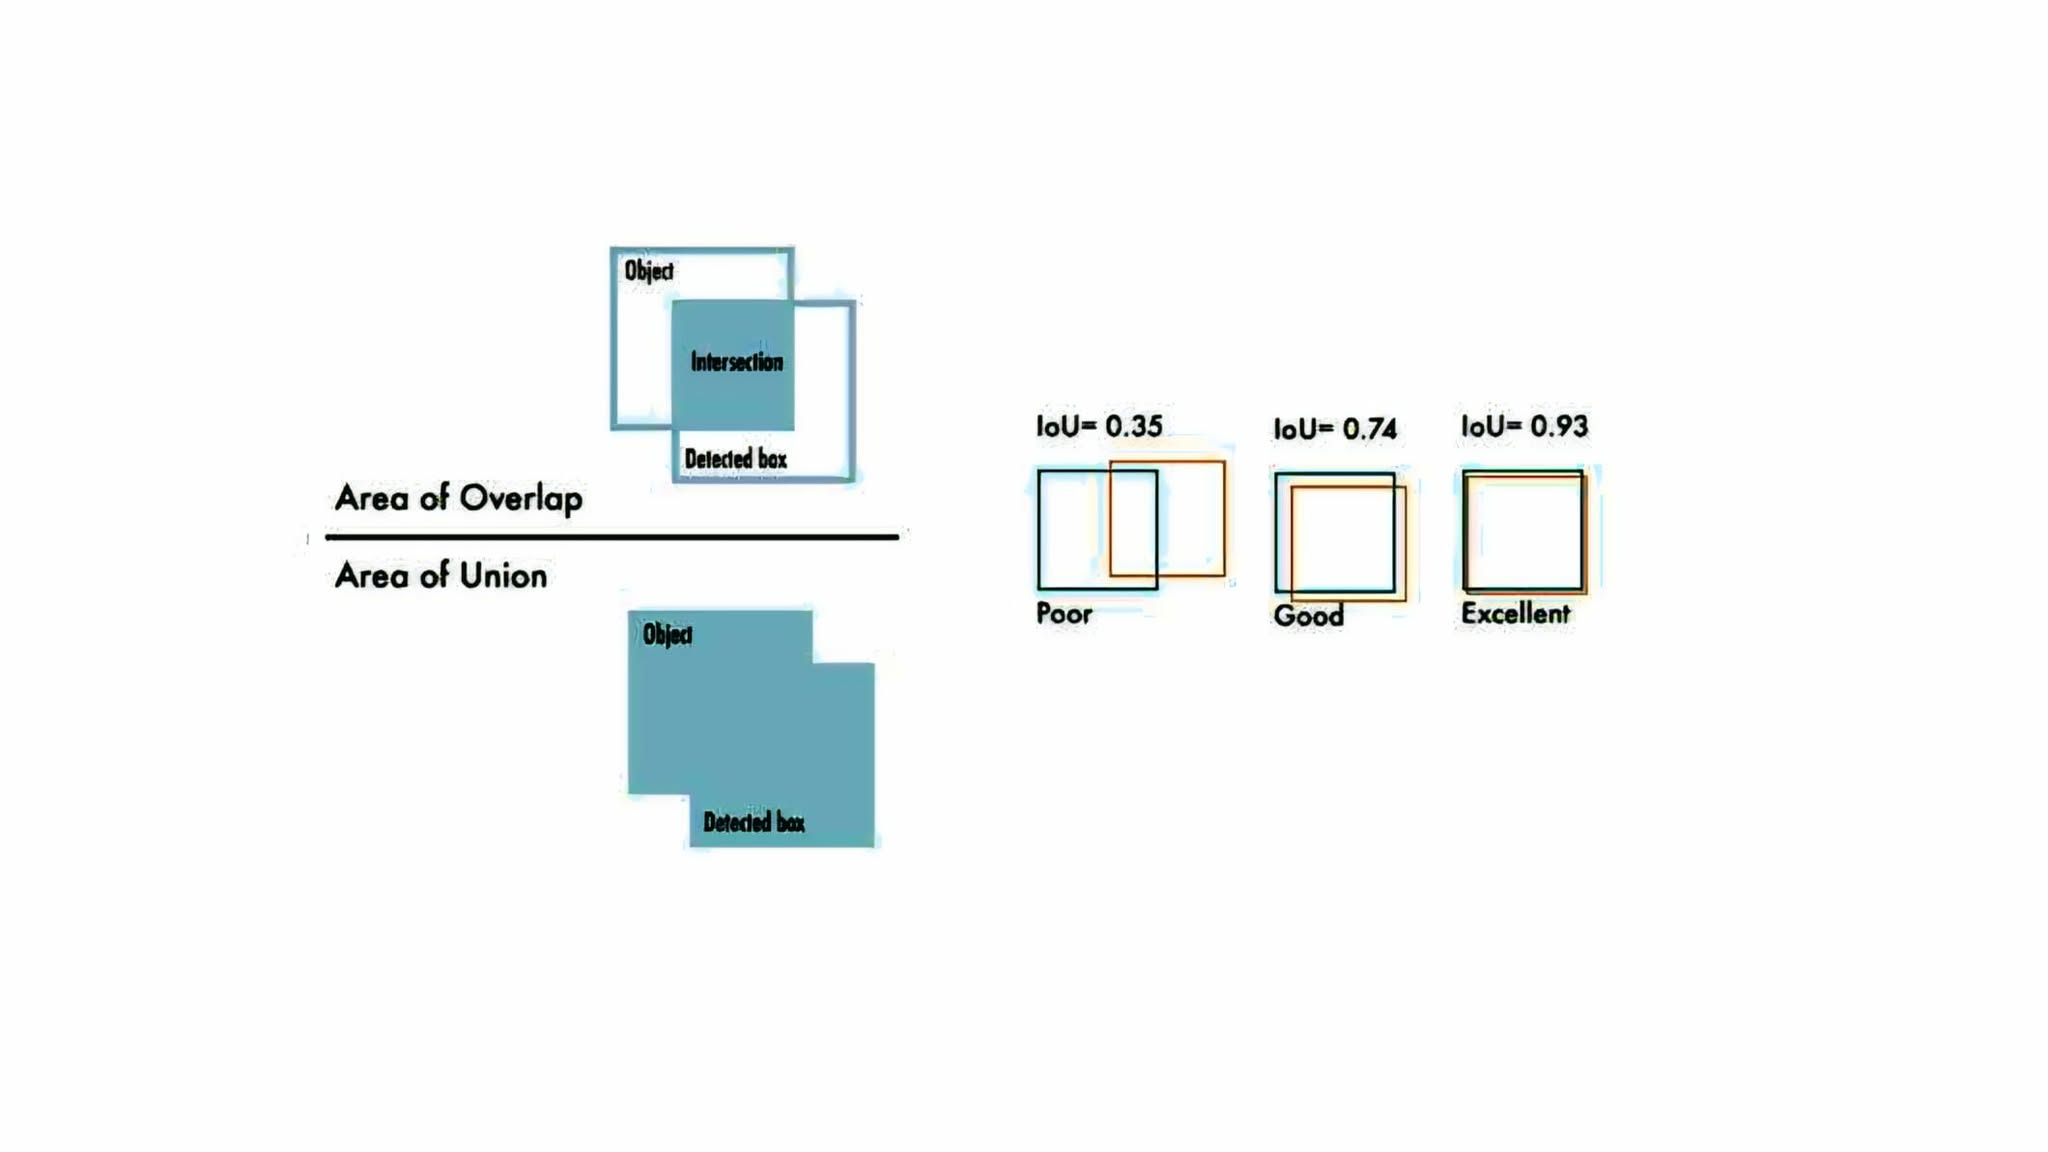
\includegraphics[width=1\textwidth]{figures/Fig 2.jpg}
    \caption{\textbf{Intersection over Union (IoU)}}
    \label{figures/Fig 2.jpg}
\end{figure}


As illustrated in Figure 2, IoU is computed by dividing the overlapping area of two boxes by their total combined area, indicating how closely the predicted box aligns with the ground truth. A higher IoU value signifies a better overlap between the predicted bounding box and the actual object. The figure further demonstrates this concept through three examples showing IoU values of 0.35, 0.74, and 0.93, corresponding to poor, good, and excellent box alignment, respectively. An IoU closer to 1 means the model has predicted the object’s location with high precision, while lower values indicate weaker performance. \cite{Terven2023}

This metric is essential in evaluating object detection models since it provides a quantitative measure of localization accuracy. For instance, many detection frameworks set a minimum IoU threshold (commonly 0.5) to determine whether a prediction is classified as a correct detection (true positive) or a missed/incorrect detection (false positive).




\subsection*{Non-Maximum Suppression (NMS)}


YOLOv8 employs Non-Maximum Suppression (NMS) to efficiently eliminate redundant bounding boxes that predict the same object. After the model generates multiple bounding boxes, NMS ranks them according to their confidence scores, identifying how likely each box contains an object. The algorithm then selects the highest-scoring box and suppresses any overlapping boxes whose Intersection over Union (IoU) with the selected box exceeds a predefined threshold. This process ensures that each detected object is represented by only one bounding box, reducing clutter and improving the clarity of detection results.
The following figure demonstrates how NMS improves detection clarity and reduces overlap.


\begin{figure}[H]
    \centering
    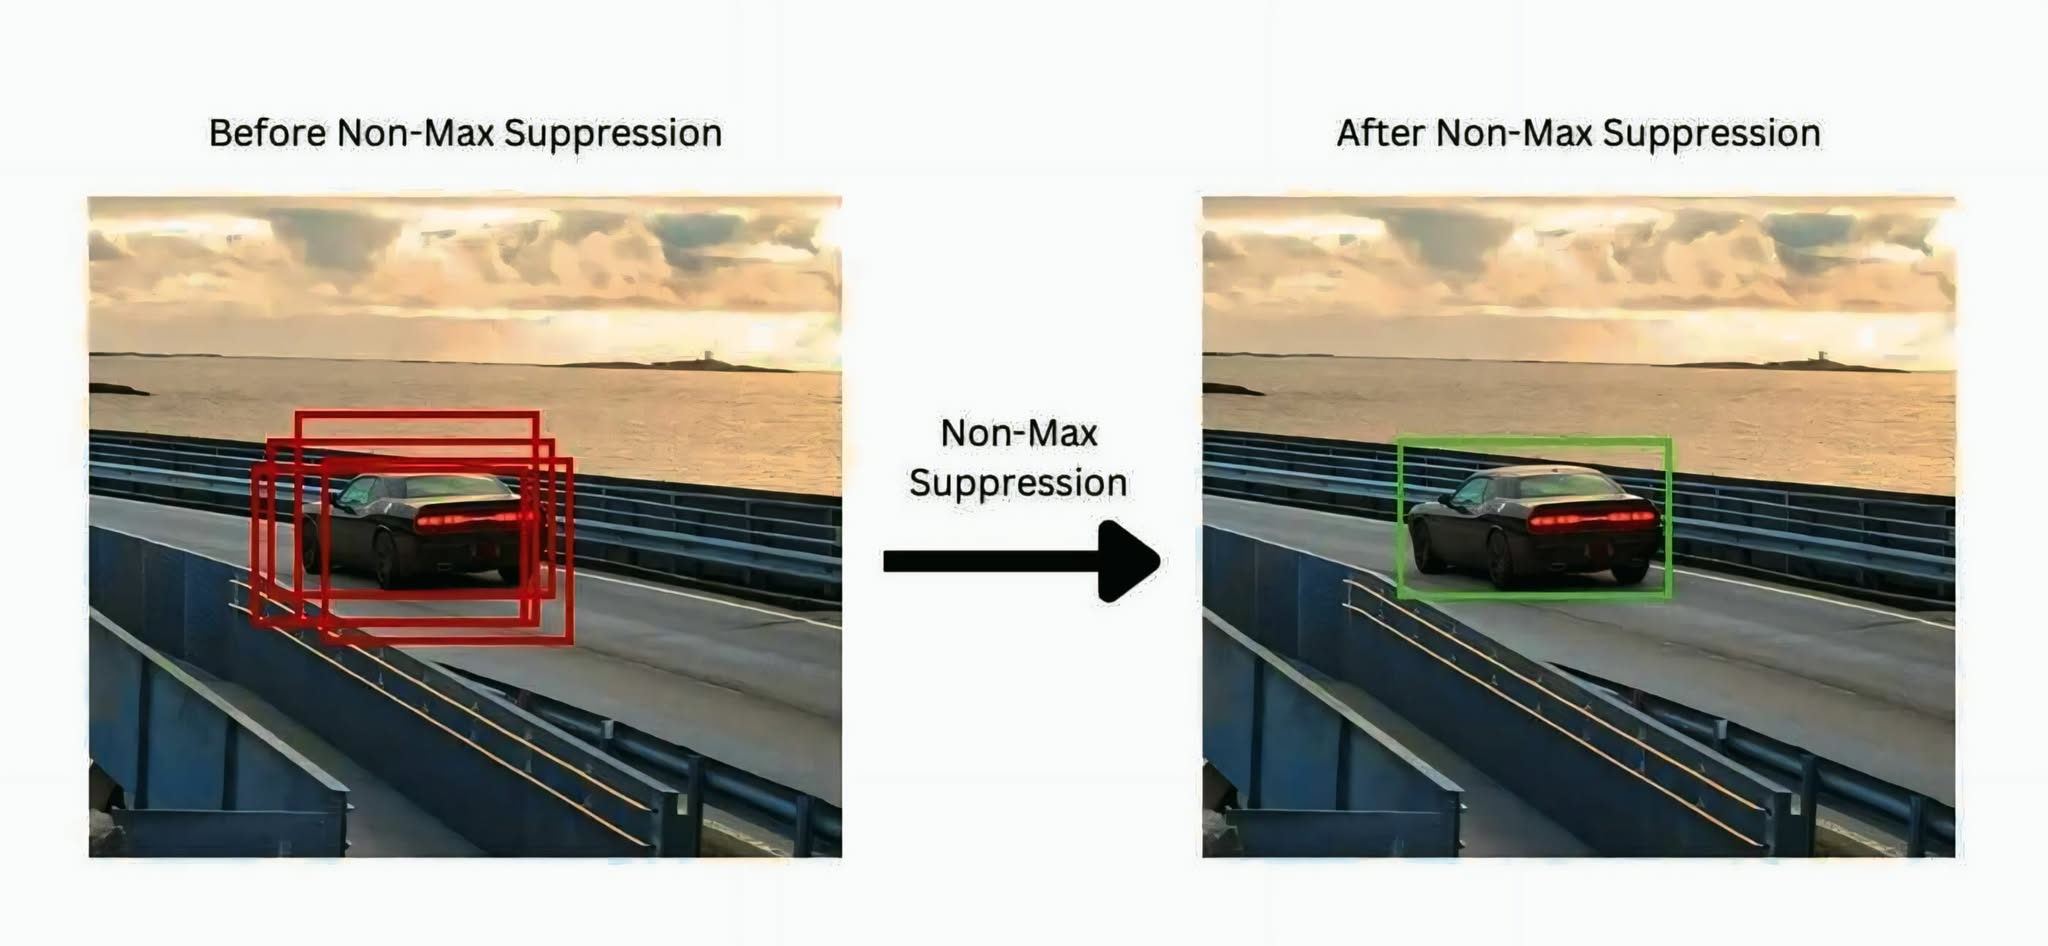
\includegraphics[width=1\textwidth]{figures/Fig 3.jpg}
    \caption{\textbf{Example of Non-Maximum Suppression }}
    \label{figures/Fig 3.jpg}
\end{figure}
Figure 3 effectively highlights the importance of Non-Maximum Suppression (NMS) in enhancing the quality of object detection results produced by YOLOv8. Without NMS, as shown in the left image, the model outputs numerous overlapping bounding boxes for a single object, which can compromise the interpretability of the results and the accuracy of object localization. The right image, after NMS is applied, displays a single, highconfidence bounding box, illustrating the algorithm’s ability to reduce redundancy and improve detection clarity. This reduction in noise not only improves precision but also lowers computational load during post-processing, making the system more efficient.


In our study, the use of NMS was particularly important in refining predictions in complex scenes involving multiple or closely spaced objects—such as identifying several riders or helmets in traffic scenarios. The figure provides clear visual evidence of how NMS strengthens both the robustness and operational efficiency of the YOLOv8-based detection pipeline \cite{ThePythonCode2021}.


\section*{Materials and Statistical Tools/Evaluation Methods}


This section provides detailed information on the materials, statistical tools, and evaluation methods employed in the development and assessment of the Helmet Compliance Detection Using Computer Vision for Safer Roads. It includes the hardware and software components, the process followed to implement the prototype, the sampling technique, the statistical tests used for performance evaluation, and the methods employed for evaluating the prototype's effectiveness.


\section*{Test Case}


The test cases briefly assess the Helmet Compliance Detection prototype’s performance by simulating a variety of real-world scenarios, including different rider counts, helmet usage patterns, lighting conditions, and visibility challenges.


These tests are designed not only to verify the accuracy of helmet and passenger detection but also to evaluate the system’s robustness and responsiveness under diverse traffic situations. By highlighting both strengths and potential areas for improvement, the test cases provide valuable insights for refining the prototype and ensuring reliable performance in practical deployment.


\begin{table}[H]
    \centering
    \caption{\textbf{Motorcycle Helmet Compliance Test Cases}}
    \label{tbl:helmetCompliance}
    \renewcommand{\arraystretch}{1} % Adjust row height
    \fontsize{11}{12}\selectfont % Readable font
    \begin{tabular}{p{1.5cm} p{5cm} p{4.5cm} p{4.5cm}}
    \hline
        \textbf{Test Case} & \textbf{Scenario Description} & \textbf{Expected Output} & \textbf{Actual Output} \\ \hline
        TC01 & 1 person riding motorcycle, wearing proper helmet & Person with proper helmet detected & Person with proper helmet detected \\
        TC02 & 1 person riding motorcycle, no helmet & Person with no helmet detected & Person with no helmet detected \\
        TC03 & 1 person riding motorcycle, helmet worn improperly & Person with wrong helmet use detected & Person with wrong helmet use detected \\
        TC04 & 1 person riding motorcycle, wearing bicycle helmet & Person with wrong helmet use detected & Person with wrong helmet use detected \\
        TC05 & 2 persons riding motorcycle, both with proper helmets & 2 persons with proper helmets detected & 2 persons with proper helmets detected \\
        TC06 & 2 persons riding motorcycle, only one with helmet & 1 proper helmet + 1 no helmet detected & 1 proper helmet + 1 no helmet detected \\
        TC07 & 2 persons riding motorcycle, both without helmets & 2 persons with no helmet detected & 2 no helmet detected \\
        TC08 & 1 person riding motorcycle, helmet worn backward & Person with wrong helmet use detected & Person with wrong helmet use detected \\
        TC09 & 3 persons riding motorcycle, all with proper helmets & Overloading violation (more than 2 riders) & 3 persons with proper helmets detected → Violation flagged \\
        TC10 & 3 persons riding motorcycle, only 1 with helmet & Overloading + helmet violations & 1 proper helmet + 2 no helmets detected \\
        TC11 & 3 persons riding motorcycle, 1 proper helmet, 1 wrong helmet, 1 no helmet & Overloading + mixed helmet violations & 3 persons detected with mixed violations \\
        TC12 & 1 person riding motorcycle, helmet is not worn (e.g., held in hand or hanging on the handlebar) & Person with wrong helmet use or no helmet detected & Person with no helmet detected \\
        TC13 & 2 adults and 1 child riding, only adults with helmets & Overloading + partial helmet usage & 2 proper helmets + 1 no helmet detected \\ \hline
    \end{tabular}
\end{table}

\noindent

The test cases for the Helmet Compliance Detection prototype cover various realistic motorcycle riding scenarios to ensure comprehensive evaluation of the system’s capabilities. TC01 confirms that the system correctly detects a single rider wearing a proper motorcycle helmet. TC02 checks whether the system properly identifies and flags a violation when a single rider has no helmet. TC03 evaluates detection when a helmet is worn improperly, such as not fastened or secured correctly, and ensures this is flagged as wrong helmet use. TC04 tests the system’s ability to differentiate and flag non-standard helmets like a bicycle helmet as improper helmet use. TC05 examines detection of two riders both wearing proper helmets, ensuring correct identification of compliant riding. TC06 validates the detection of partial compliance, where only one of two riders wears a helmet, ensuring the system outputs one proper helmet and one no helmet. 

Also, TC07 confirms detection when both riders have no helmets, expecting the system to identify both violations. TC08 tests for improper helmet use when a rider wears the helmet backward, which should be detected as wrong helmet use. TC09 checks overloading detection, where three riders are on a motorcycle, all with proper helmets, but a violation is flagged due to exceeding the legal number of passengers. TC10 ensures the system detects both overloading and missing helmets when only one of three riders wears a proper helmet. TC11 verifies detection of mixed violations among three riders—one with a proper helmet, one with wrong helmet use, and one with no helmet—along with overloading. TC12 evaluates if the system correctly identifies violations when the helmet is present but not worn, such as when carried in hand or placed on the motorcycle. Finally, TC13 tests overloading combined with partial helmet use when two adults wear helmets but a child passenger does not. Overall, these test cases demonstrate the prototype’s ability to detect proper helmet use, identify different violation scenarios, and monitor overloading, ensuring road safety compliance and pinpointing areas for refinement.


\section*{Instrument}


    The research tool used by the researchers to carry out the study was described in this section.


\subsection*{Dataset}


The dataset used in this study is a custom dataset created and annotated by the researchers. It contains annotated images for four classes: motorcycle, person with no helmet, person with proper helmet, and person with wrong helmet use. This dataset was specifically collected to align with the goals of the prototype, particularly in monitoring helmet compliance and identifying motorcycles using YOLOv8. Passenger counting, on the other hand, is not included in the dataset since this feature is implemented directly in the system’s code by checking the number of detected persons per motorcycle and flagging a violation if more than two riders are present. To enhance the dataset, images were carefully collected to capture various real-world scenarios, particularly different cases of helmet compliance and violation. This ensures that the trained model can reliably distinguish between proper helmet use, no helmet use, and wrong helmet use, while also maintaining accurate motorcycle detection.

% Row 1
\begin{figure}[H]
    \centering
    \begin{subfigure}{0.45\textwidth}
        \centering
        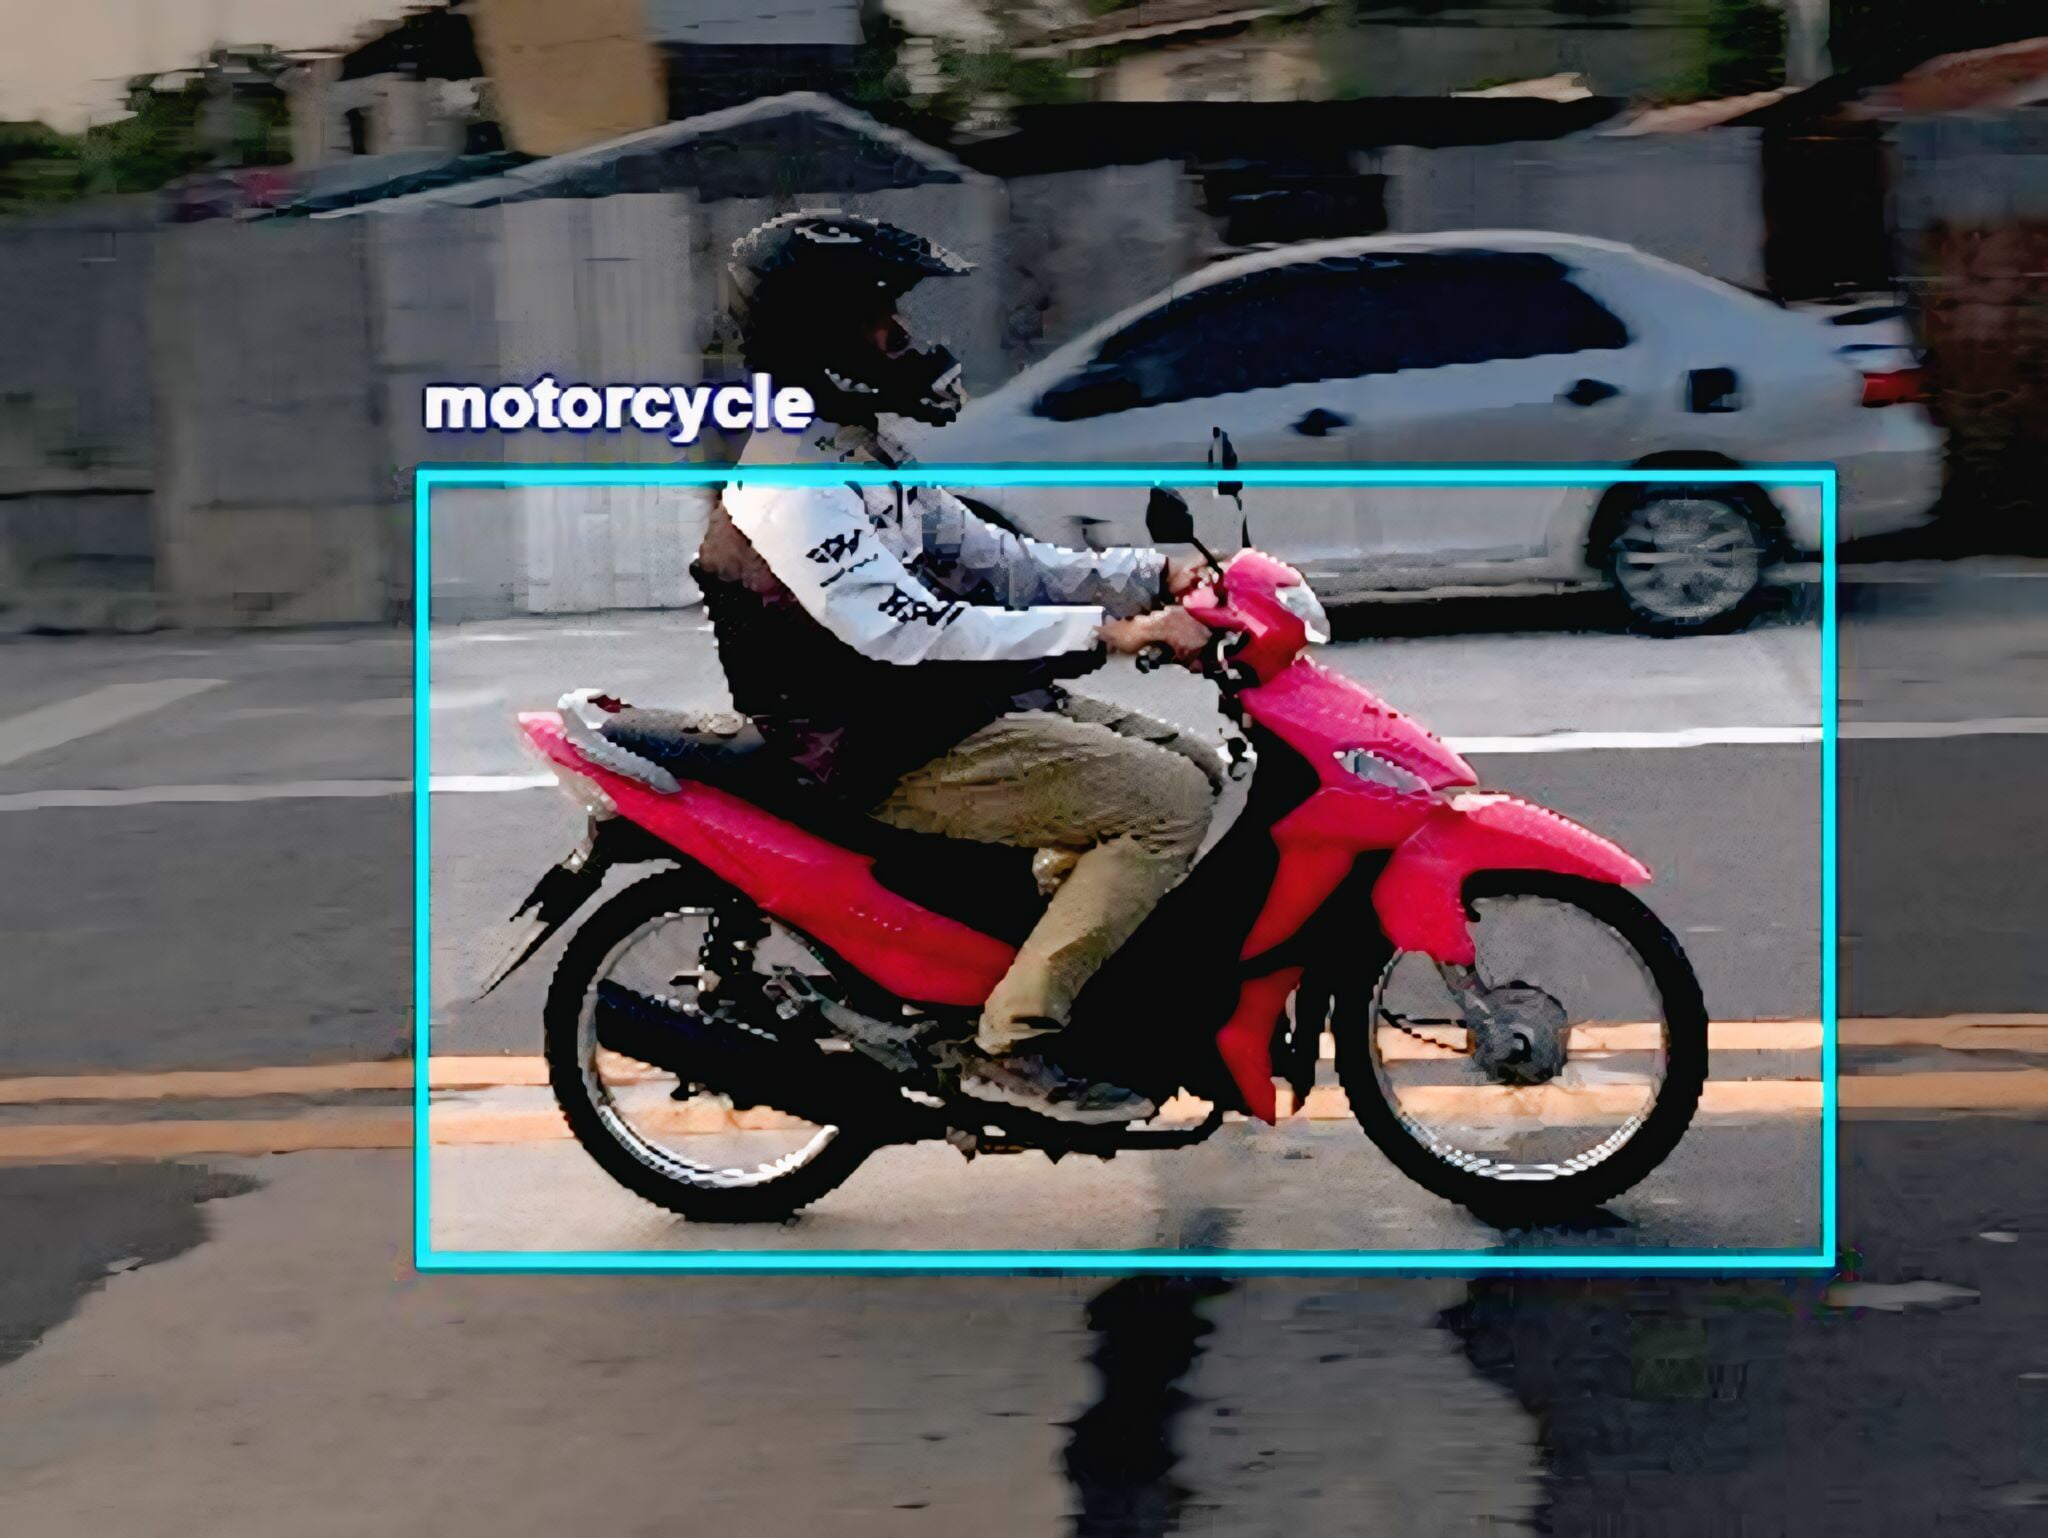
\includegraphics[width=\linewidth]{figures/Fig 4a.jpg}
        \caption{motorcycle}
        \label{fig:4a}
    \end{subfigure}
    \hfill
    \begin{subfigure}{0.45\textwidth}
        \centering
        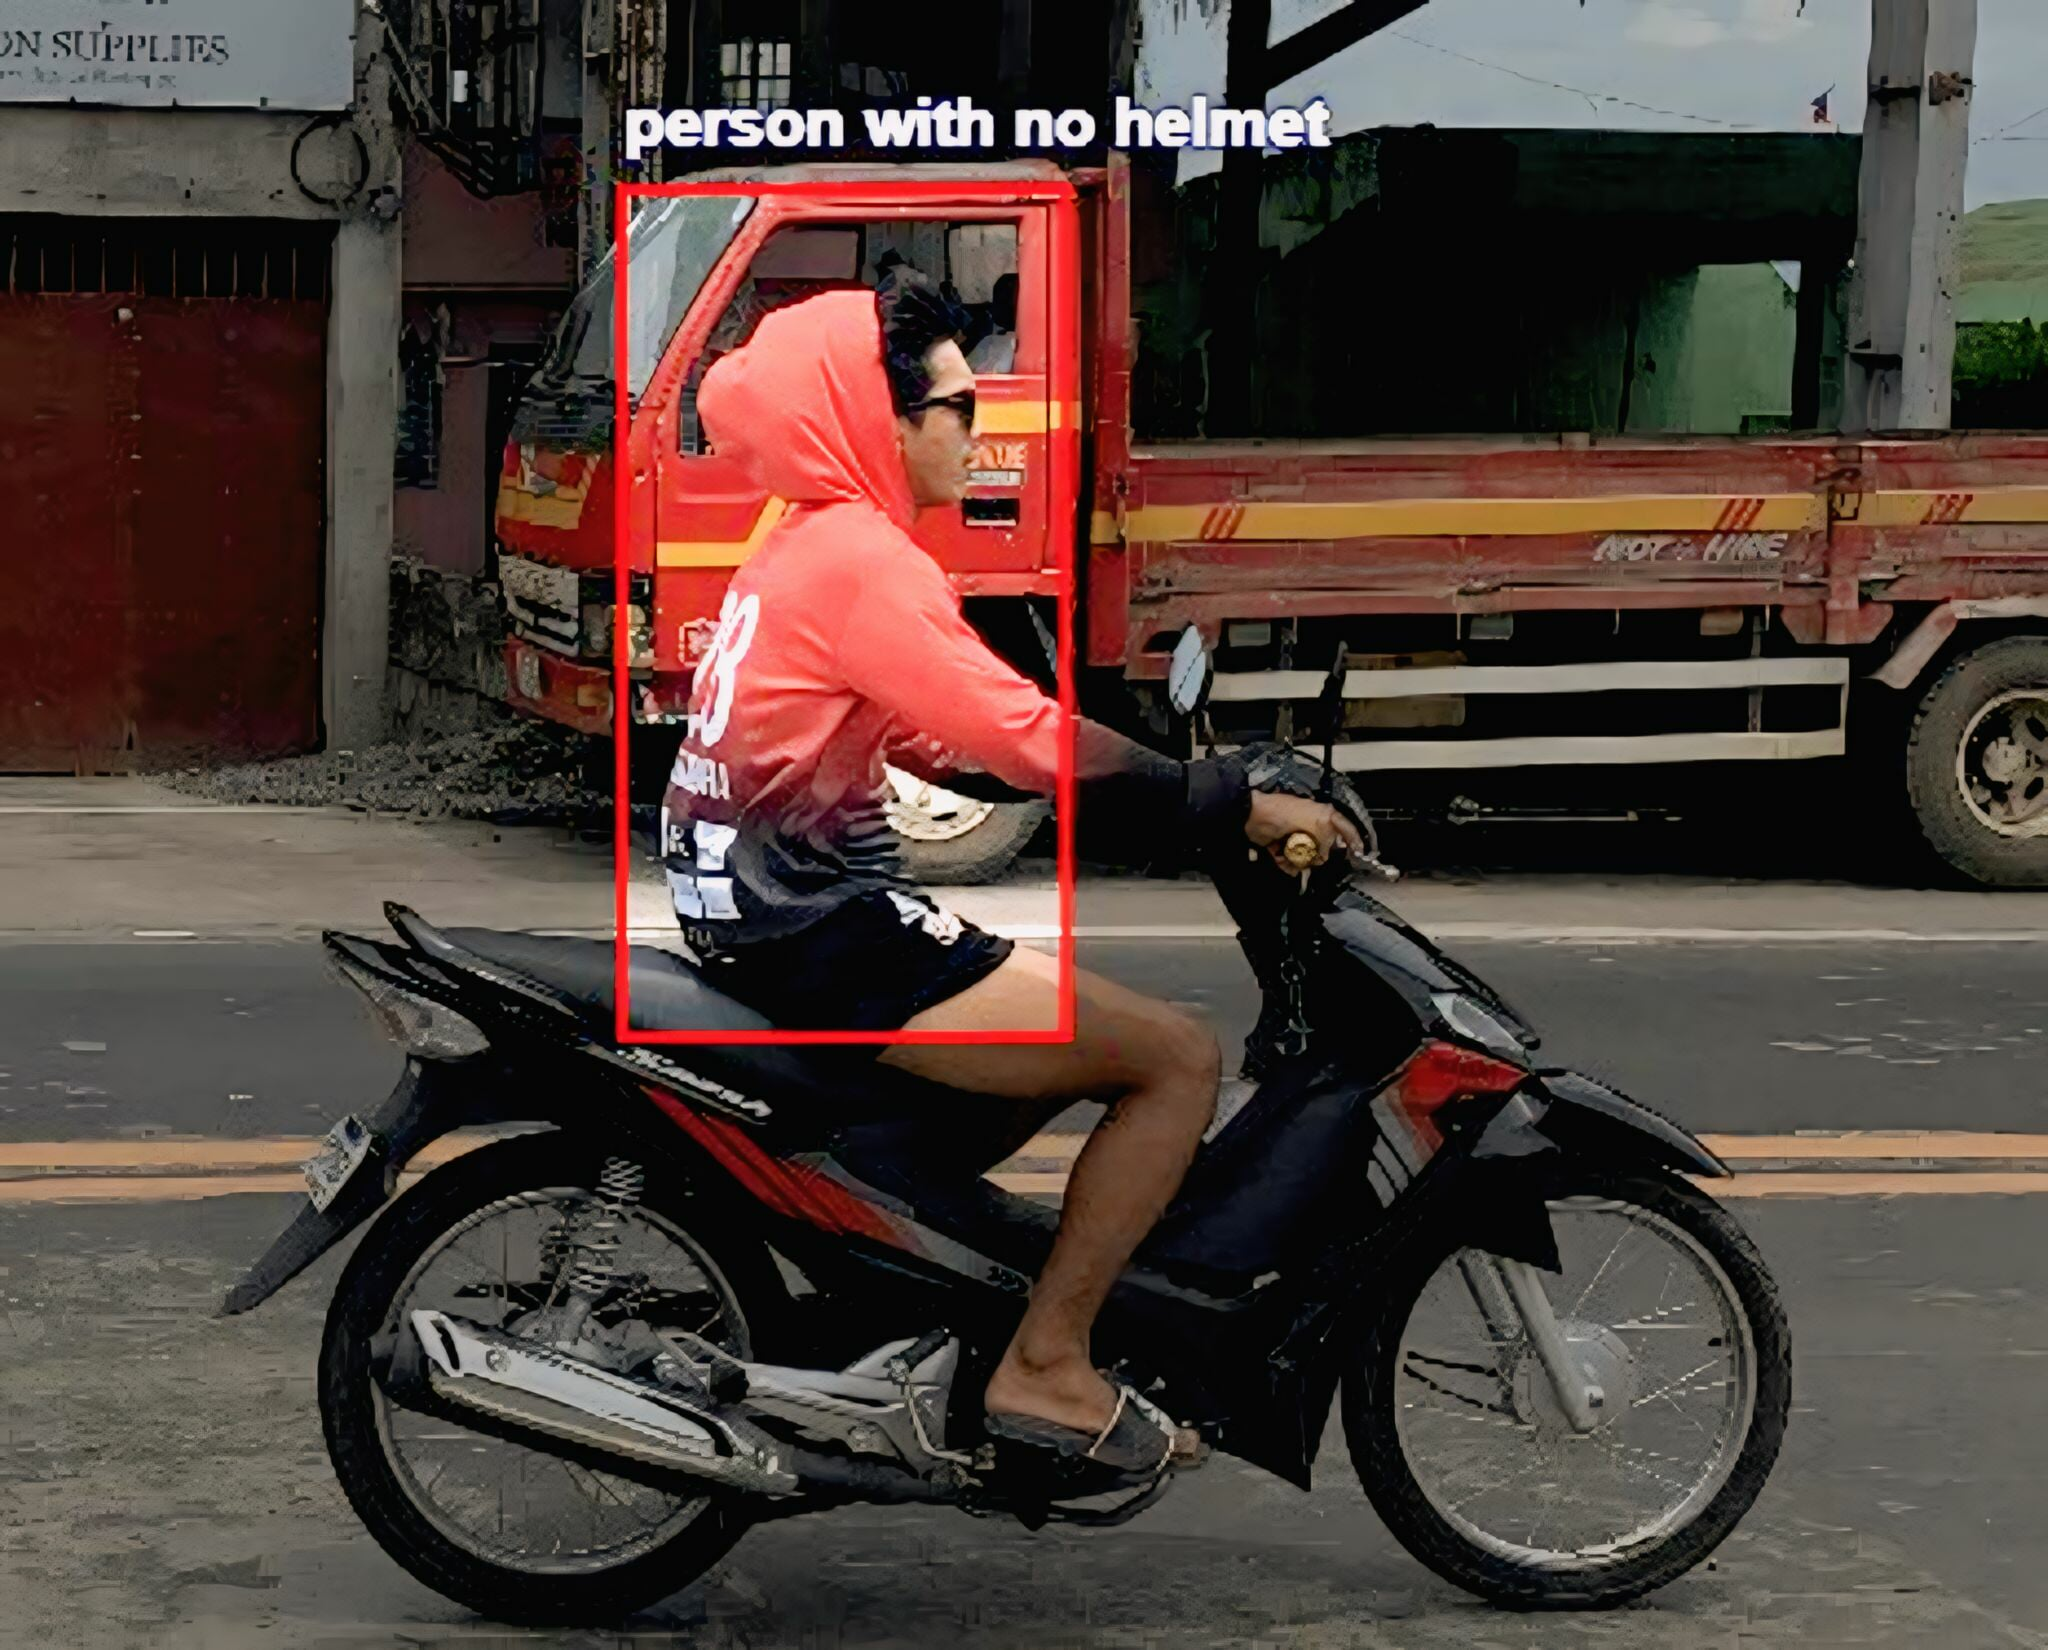
\includegraphics[width=\linewidth]{figures/Fig 4b.jpg}
        \caption{person with no helmet}
        \label{fig:4b}
    \end{subfigure}
    \label{fig:dataset_row1}
\end{figure}

% Row 2
\begin{figure}[H]
    \centering
    \begin{subfigure}{0.45\textwidth}
        \centering
        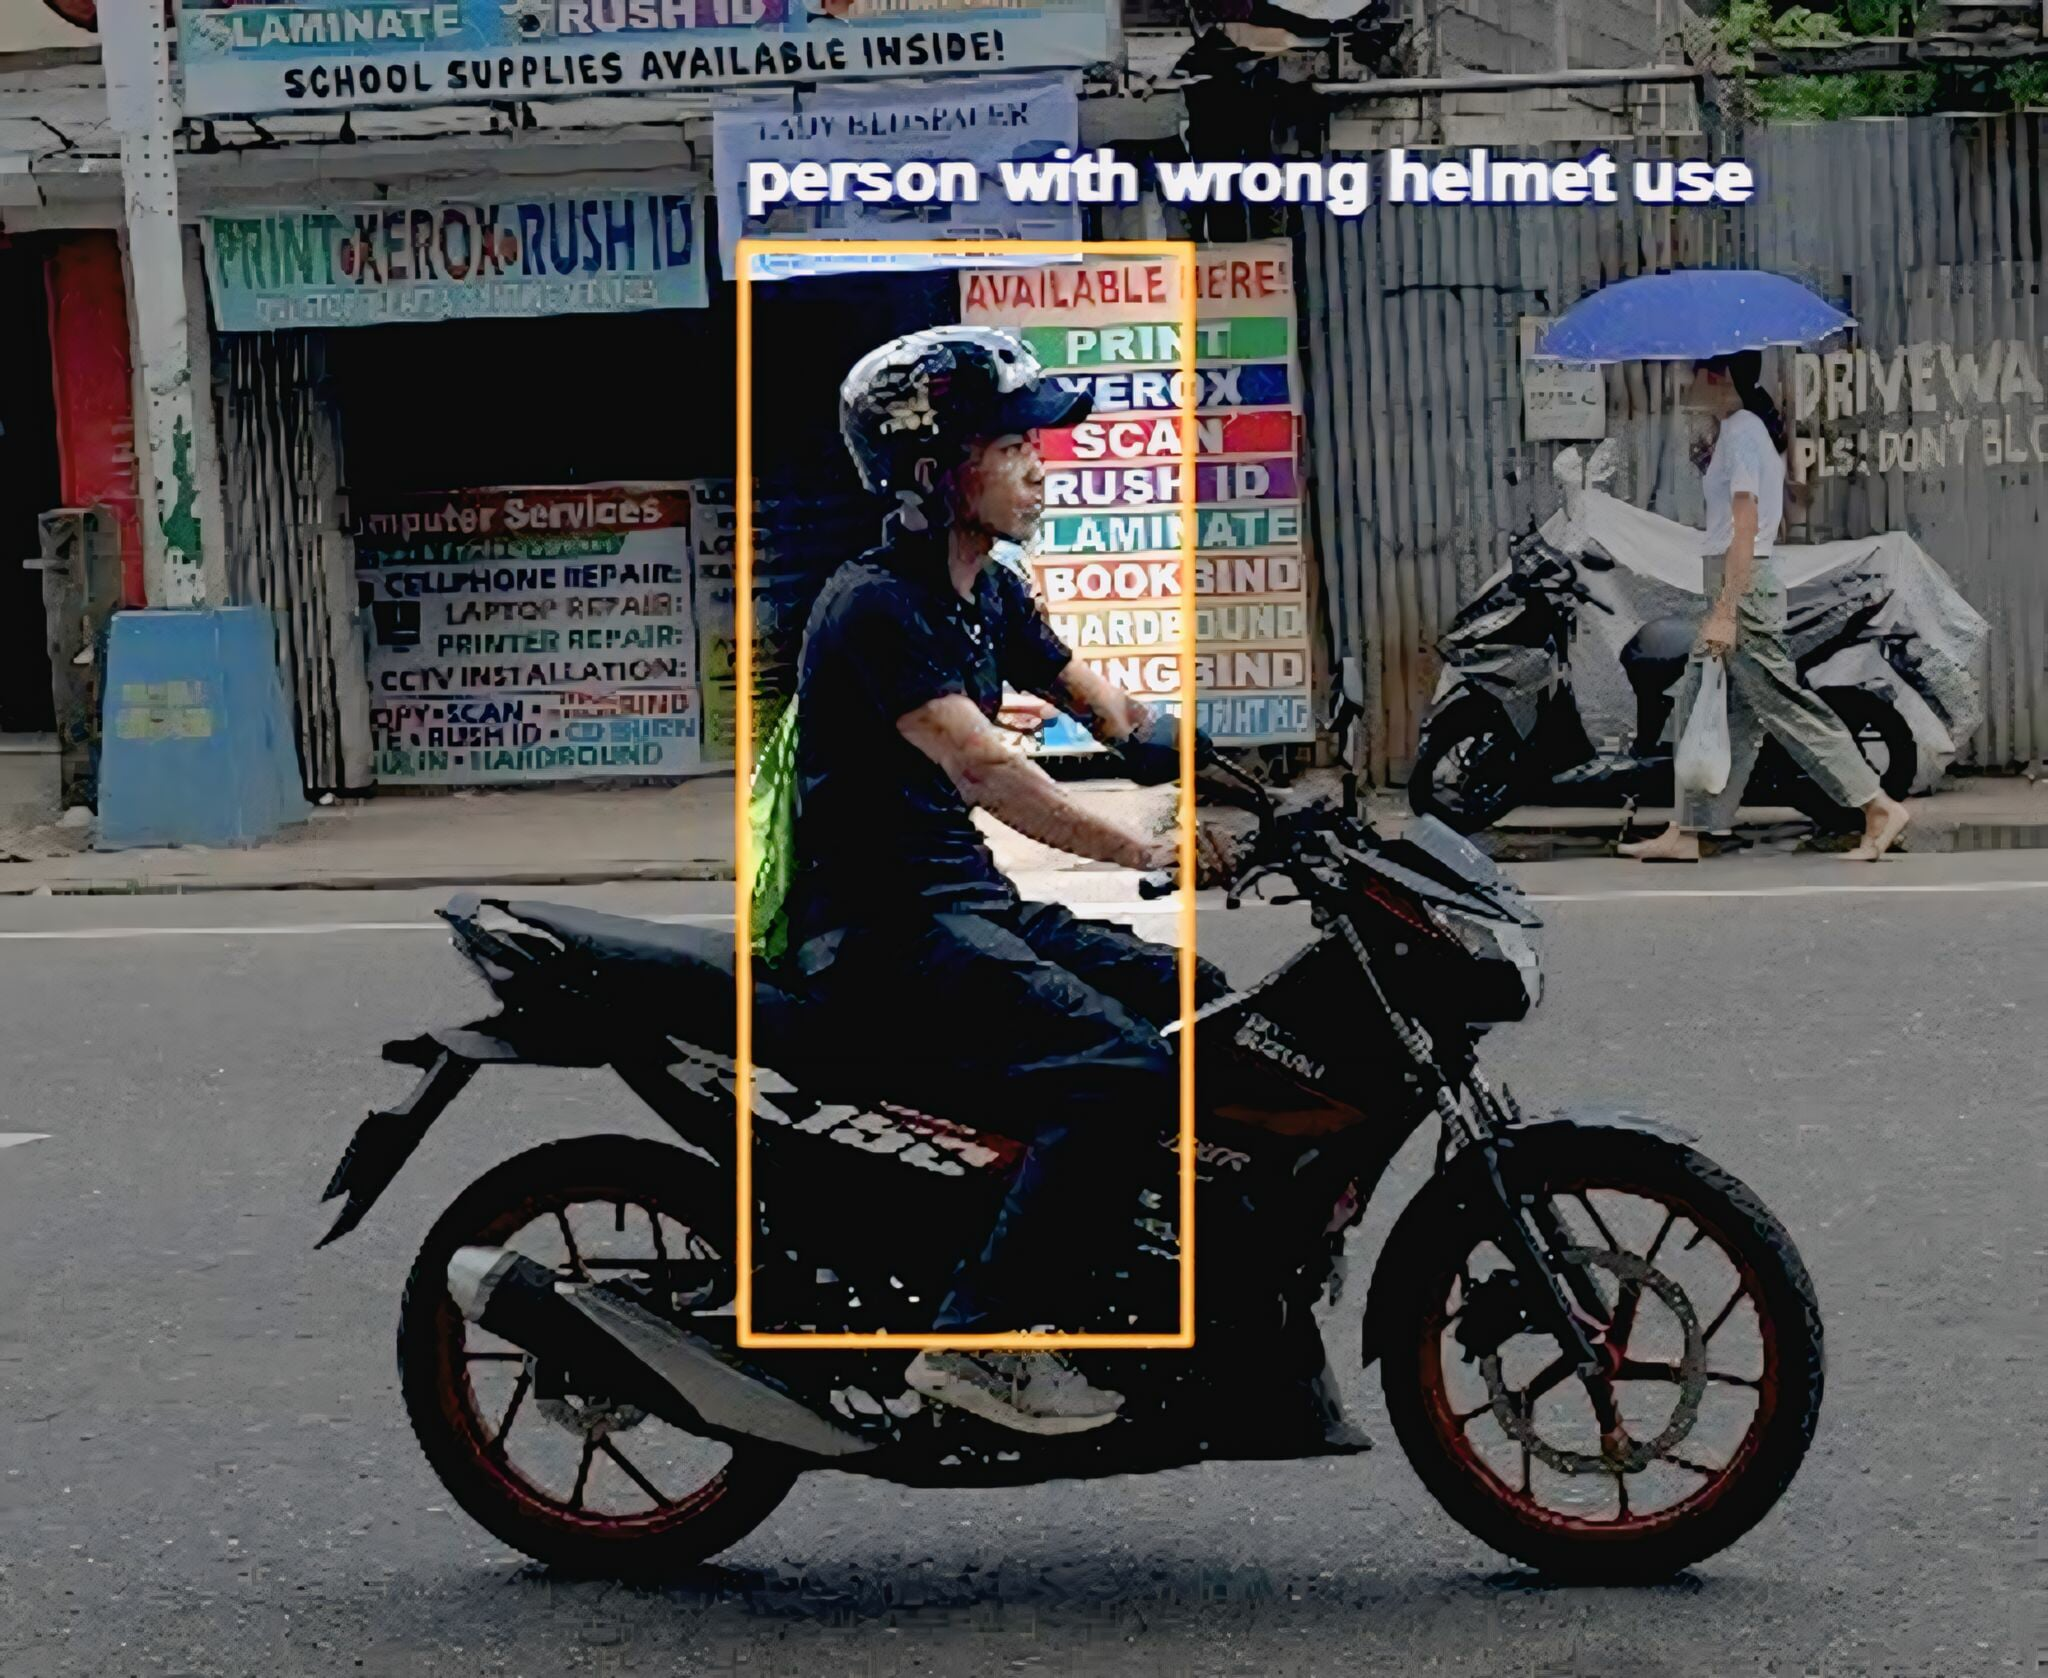
\includegraphics[width=\linewidth]{figures/Fig 4c.jpg}
        \caption{person with wrong helmet use}
        \label{fig:4c}
    \end{subfigure}
    \hfill
    \begin{subfigure}{0.45\textwidth}
        \centering
        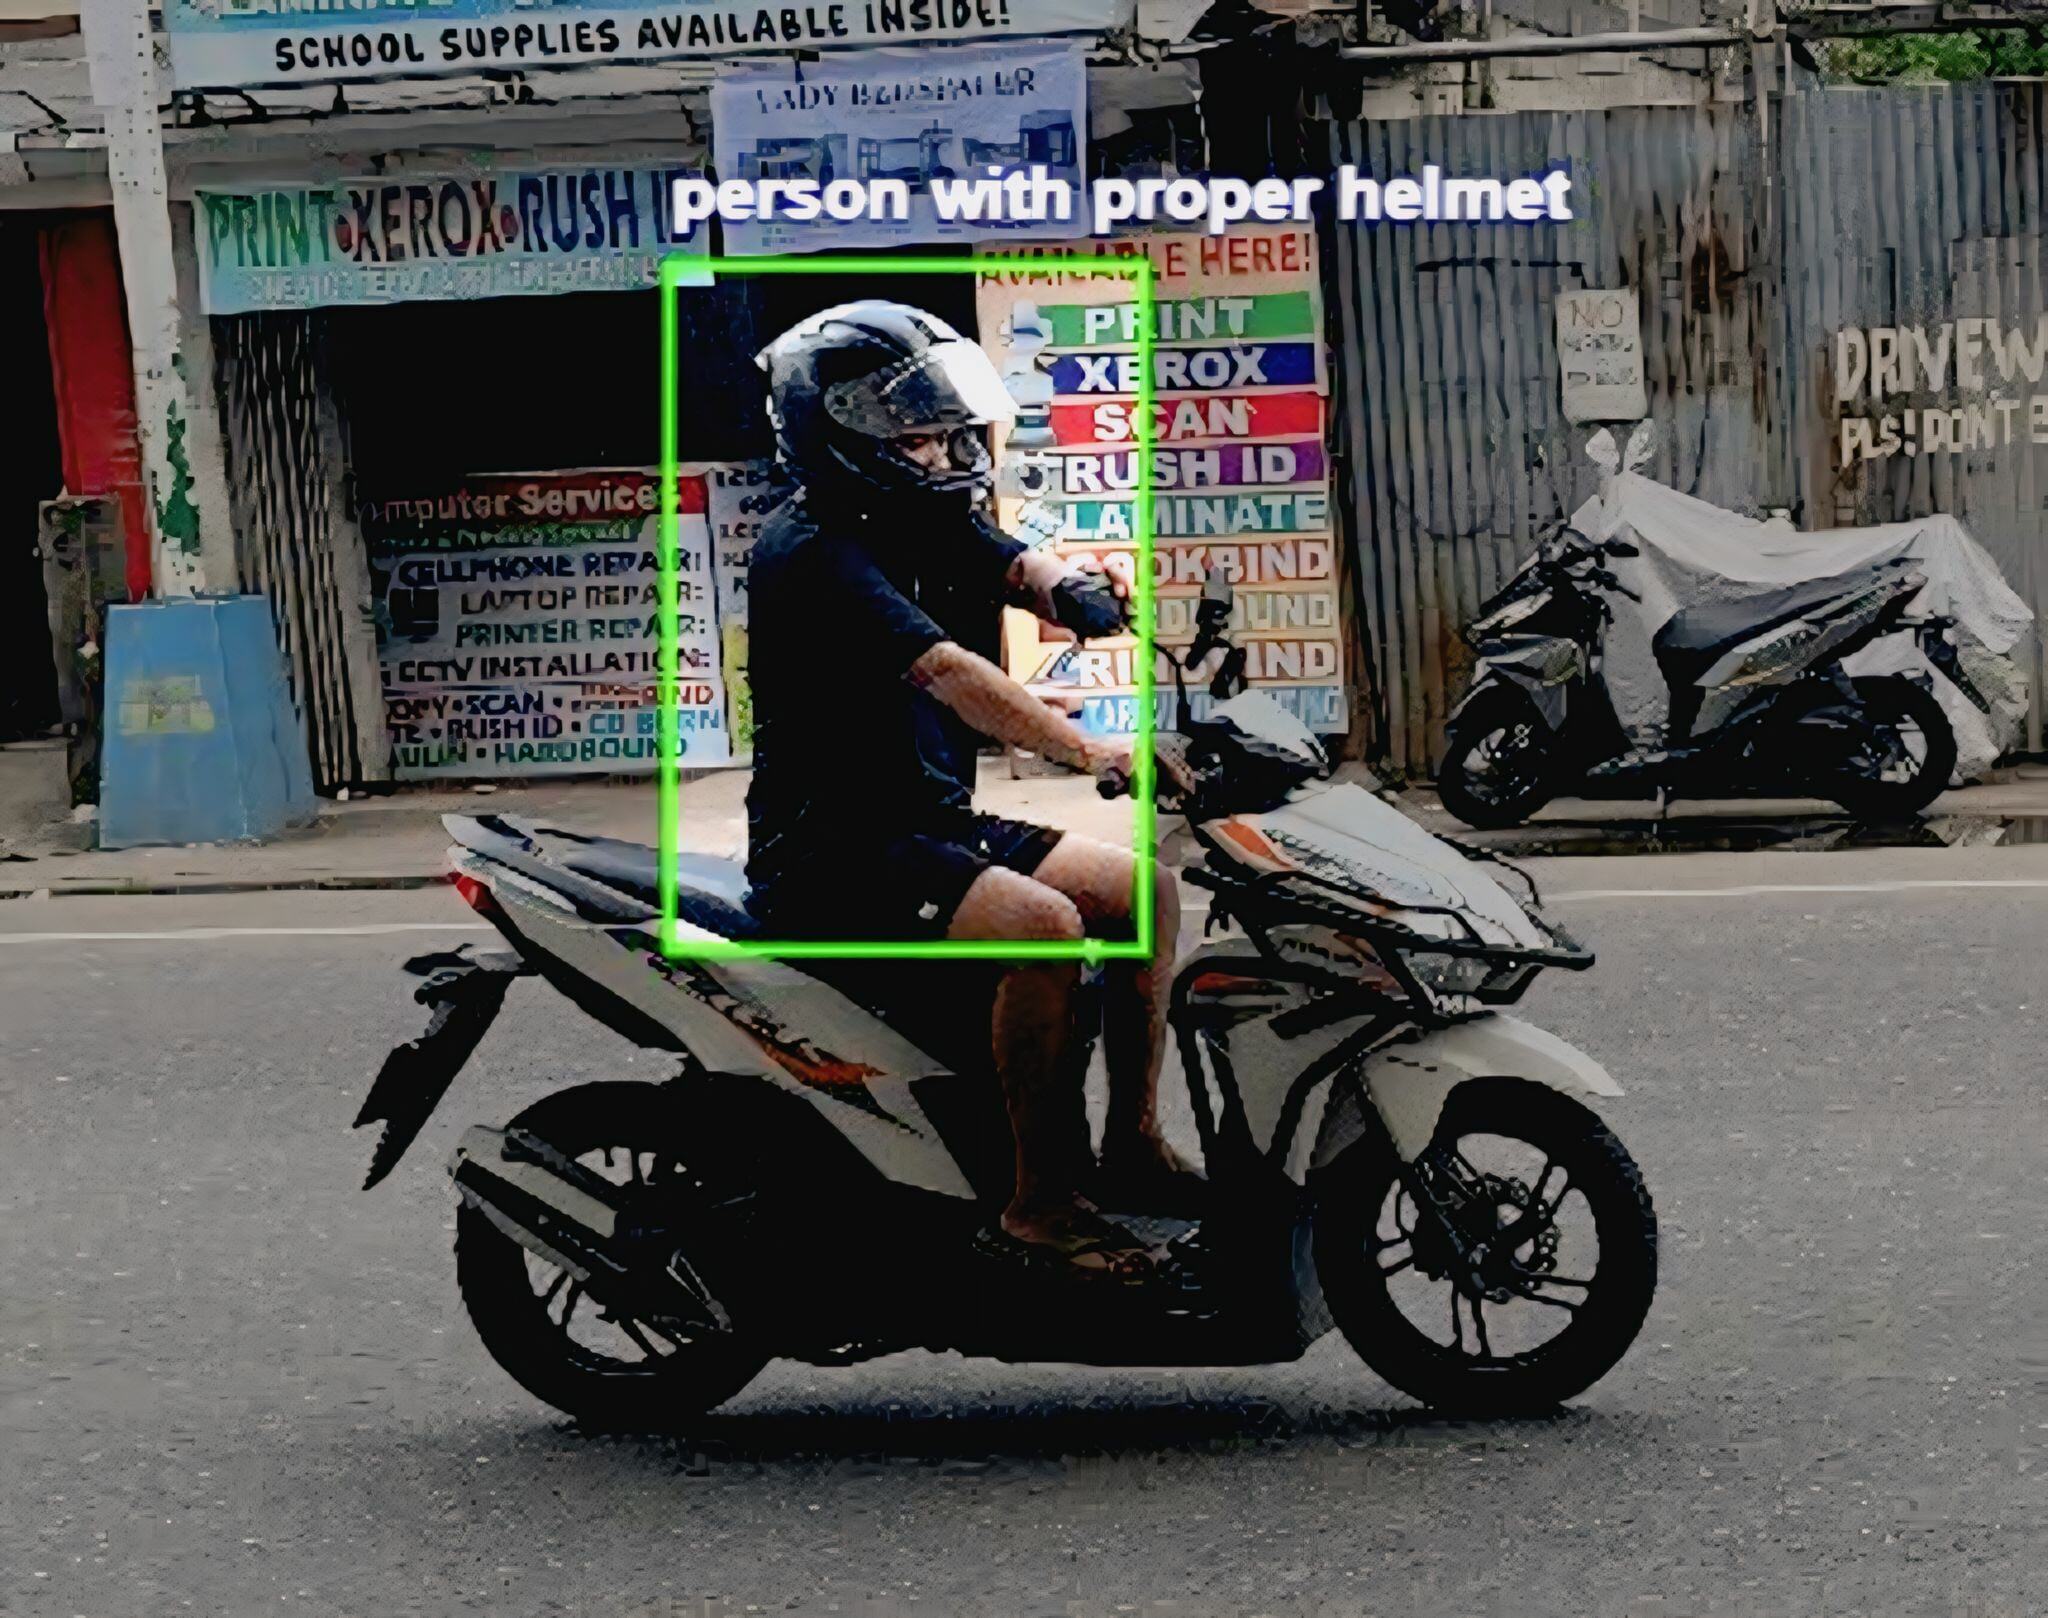
\includegraphics[width=\linewidth]{figures/Fig 4d.jpg}
        \caption{person with proper helmet}
        \label{fig:4d}
    \end{subfigure}
    \caption{\textbf{Samples of Dataset}}
    \label{fig:dataset_row2}
\end{figure}

\noindent

The image above illustrates the Helmet Compliance Detection Using Computer Vision prototype trained on a unified dataset with four main classes: (a) Motorcycle, which enables the system to correctly identify and recognize motorcycles on the road; (b) Person with No Helmet, which allows the system to detect riders who are not wearing helmets (c) Person with Wrong Helmet Use, which identifies riders wearing helmets incorrectly, and (d) Person with Proper Helmet, which confirms compliance with safety regulations. These four classes help the prototype detect motorcycles, identify helmet compliance, and overloading.
Additionally, a separate Vehicle Filtering Dataset is used, which contains a single class labeled as “not motorcycle.” This dataset enables the prototype to filter out non-motorcycle vehicles before proceeding to helmet and passenger compliance detection, thereby ensuring more accurate and reliable results.



\section*{Procedure / Process}


\subsection{Data Collection} \\
Video footage is live along the Nabua Highway under various traffic and lighting conditions to capture real-world motorcycle scenarios. These videos serve as the primary input for detecting helmet usage.

\subsection {Data Preprocessing} \\
The collected data were processed using OpenCV to resize frames, enhance image quality, and normalize the input. This step ensures that the data is clean and ready for analysis by the detection model.

\subsection {Model Training} \\
The YOLOv8 model was trained using labeled data to identify whether the rider and pas- senger are wearing helmets. The model was tested with a separate dataset to ensure its accuracy in helmet detection.

\subsection {Vehicle Filtering} \\
As vehicles pass through the camera, the system first filters and detects whether the vehicle is a motorcycle. Only motorcycles are analyzed for helmet compliance.

\subsection {Helmet Detection} \\
Once a target vehicle is identified as a motorcycle, the system proceeds to detect whether the rider is wearing a helmet. If a passenger is also detected, the system checks whether the passenger is wearing a helmet or merely holding one or with wrong helmet use.

\subsection{Real-Time Monitoring}
All detection processes run in real time, ensuring continuous monitoring and immediate feedback on helmet law compliance.

\subsection {Real-time Violation Alert} \\
If any person on the motorcycle (rider or passenger) is detected without a helmet or with wrong helmet use, a real- time violation alert pops up on the monitoring screen. This allows for immediate awareness and potential enforcement.


\begin{figure}[H]
    \centering
    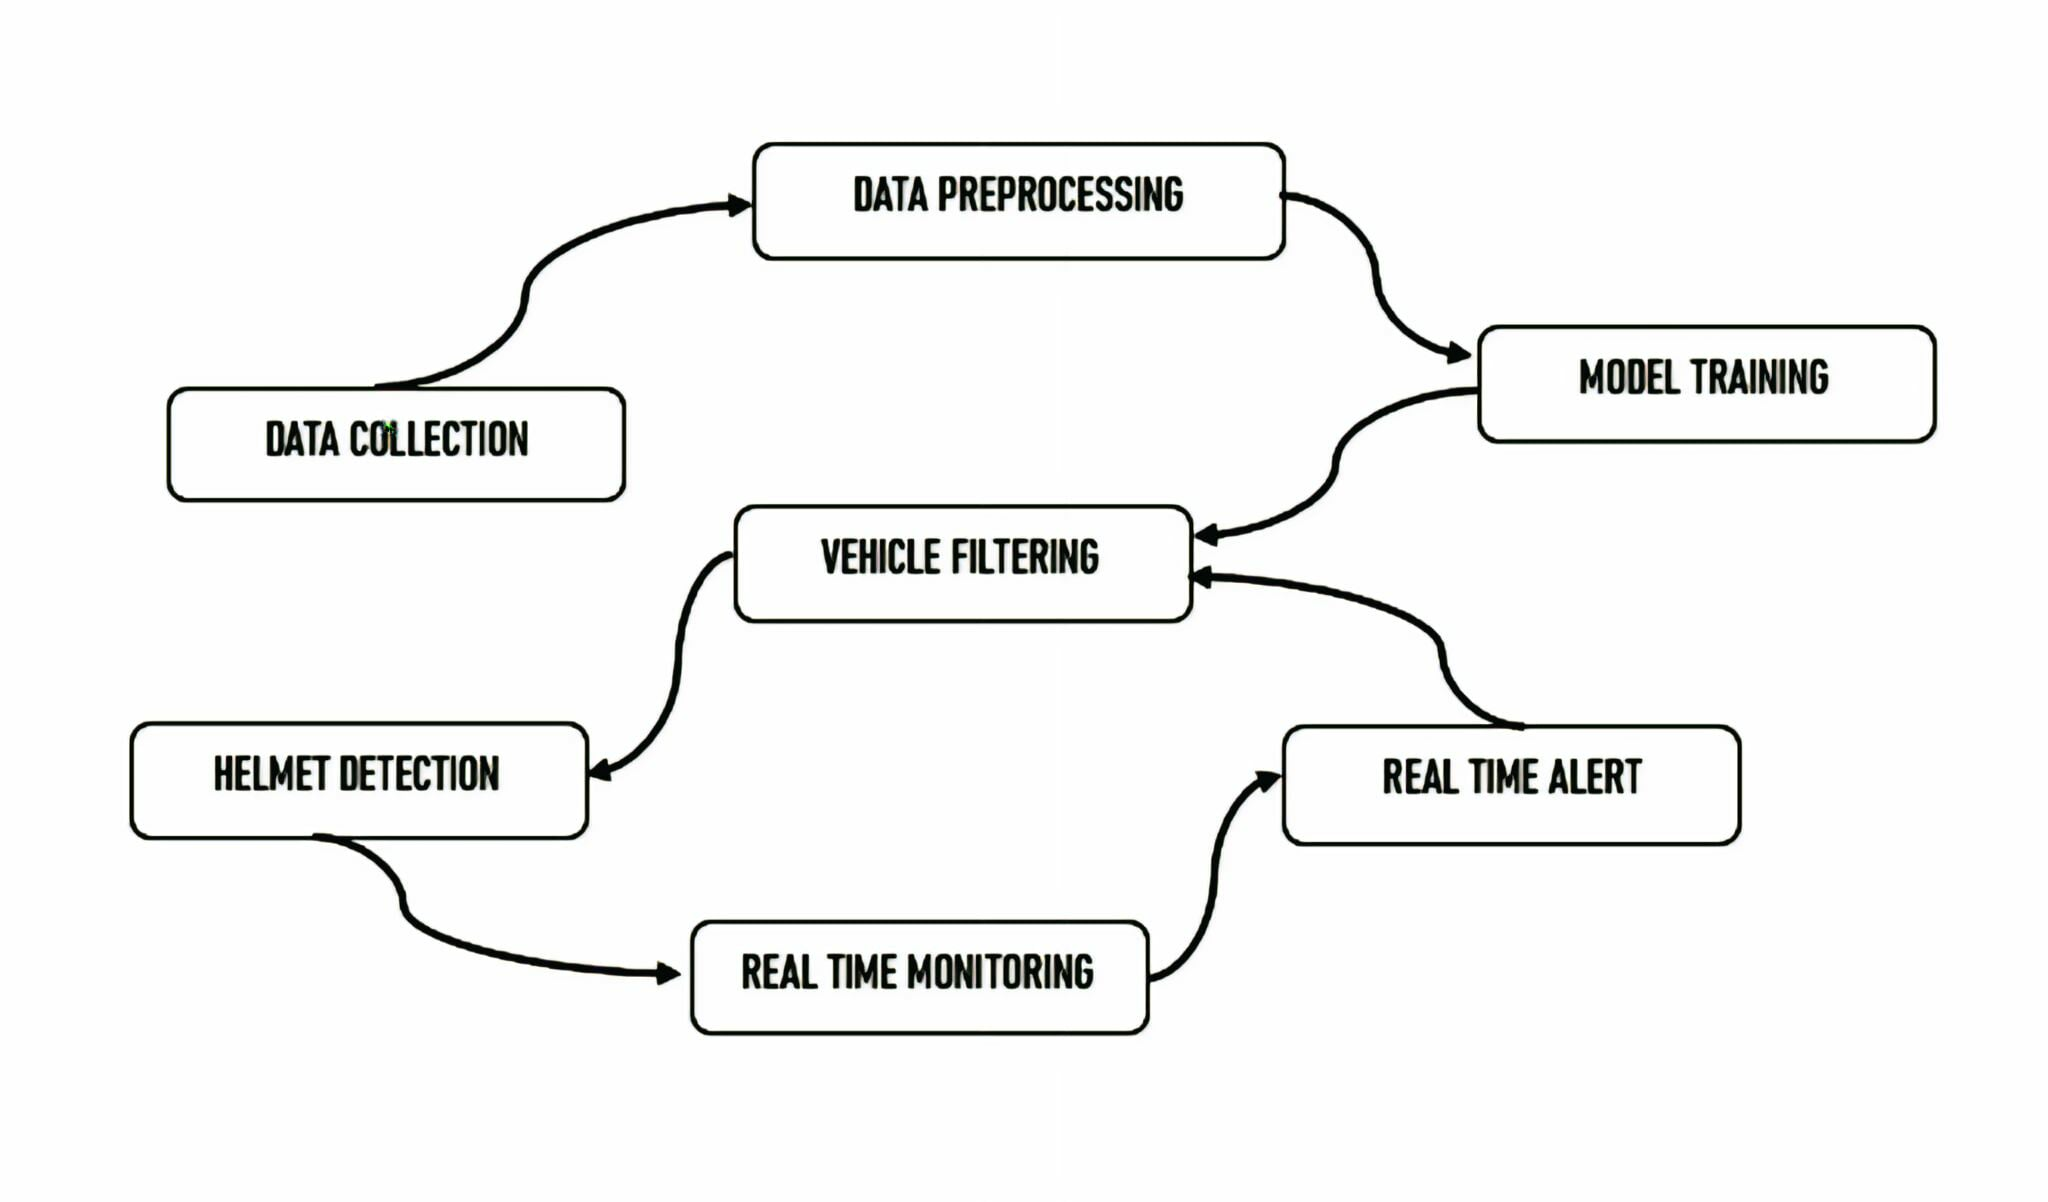
\includegraphics[width=0.9\textwidth]{figures/Fig 5.jpg}
    \caption{\textbf{Prototype of Flowchart}}
    \label{figures/Fig 5.jpg}
\end{figure}

\noindent
The diagram presents a real-time helmet detection system workflow. It starts with video data collection and preprocessing to prepare frames for analysis. A YOLOv8 model is trained to detect helmets on motorcycle riders and passengers. 
During real-time operation, the system filters vehicles to focus on motorcycles, then checks for helmet compliance. If a violation is found, an alert is triggered and displayed and saves a video clip of the violation. The system continuously monitors and loops back to analyze the next vehicle, ensuring ongoing detection and enforcement of helmet laws.

\section*{Normalized Value}
The normalized value is used to standardize the raw user feedback scores, transforming them into a range between 0 and 1. The formula for normalization is:


\begin{equation}
\text{Normalized Value} = \frac{X - \min(X)}{\max(X) - \min(X)}
\end{equation}


\noindent Where:  
\begin{itemize}
    \item $X$ is the raw score obtained from user feedback.
    \item $\min(X)$ is the minimum possible value (typically 0.0).
    \item $\max(X)$ is the maximum possible value (typically 1.0).
\end{itemize}


After applying this formula, the normalized values are mapped to the ranges in Table 3, allowing the responses to be categorized according to satisfaction levels. This normalization ensures that the feedback is consistent and comparable across different system components. The final categorized feedback provides a clear understanding of user satisfaction and highlights areas where the prototype may need improvement or refinement.


\section*{Evaluation Method}
To evaluate the performance of the proposed Helmet Compliance Detection Using Computer Vision for Safer Roads, several standard evaluation metrics were utilized. These metrics assess the system’s accuracy in detecting helmet usage, counting passengers, and identifying violations in real time. The evaluation was based on comparing the model’s predictions against manually annotated ground truth data using test video segments.


\section*{Accuracy}

Accuracy measures the overall effectiveness of the prototype by calculating the percentage of correctly identified objects (motorcycles, helmets and overloading violations) as well as correctly filtered non-motorcycle vehicles. It provides a general view of the system’s performance across all detection tasks.

\begin{equation}
    \text{Accuracy} = \frac{TP + TN}{TP + TN + FP + FN}
\end{equation}

Where:
\begin{itemize}
    \item \textbf{TP (True Positives):} Instances where motorcycles, helmets, passengers, overloading violations, or non-motorcycles were correctly detected or filtered.

    \item \textbf{TN (True Negatives):} Instances where non-violations or non-motorcycle objects were correctly ignored.

    \item \textbf{FP (False Positives):} Instances where incorrect objects were detected, such as misclassifying a non-motorcycle as a motorcycle or falsely detecting a helmet violation.

    \item \textbf{FN (False Negatives):} Instances where motorcycles, helmets, passengers, overloading violations, or non-motorcycles were missed.
\end{itemize}



    \item \textbf{Precision:}  Precision measures the ability of the system to correctly identify positive cases out of all instances that the system marked as positive. In the context of this prototype, it evaluates how often the model correctly identifies helmet violations, motorcycles, or overloading instances compared to the total number of predicted positives. A high precision indicates that the system rarely produces false alarms.
    \begin{equation}
        Precision = \frac{TP}{TP + FP}
        \label{eq:precision}
    \end{equation}
    Where:
    \begin{itemize}
        \item $TP$ = True Positives (correct helmet detections)
        \item $FP$ = False Positives (incorrect helmet detections)
    \end{itemize}


    \item \textbf{Recall:}  Recall evaluates the ability of the system to detect all actual positive cases. For example, it shows how effectively the prototype detects all instances of helmet violations, motorcycles, or overloading occurrences from the ground truth. A high recall ensures that the system captures most or all violations, minimizing missed detections.
    \begin{equation}
        Recall = \frac{TP}{TP + FN}
        \label{eq:recall}
    \end{equation}
    Where:
    \begin{itemize}
        \item $TP$ = True Positives (correct helmet detections)
        \item $FN$ = False Negatives (missed helmet detections)
    \end{itemize}


    \item \textbf{F1-Score:}  The F1-Score is the harmonic mean of precision and recall, providing a single metric that balances the system’s ability to avoid false positives while capturing as many true positives as possible. It is particularly useful when the dataset is unbalanced, such as when the number of riders violating helmet rules is much smaller than the number of riders wearing helmets correctly.
    \begin{equation}
        F1\text{-}Score = \frac{2 \times Precision \times Recall}{Precision + Recall}
        \label{eq:f1score}
    \end{equation}
\end{itemize}


\section*{Mean Average Precision (mAP)}


 Mean Average Precision (mAP) evaluates both the precision and localization accuracy of the predicted bounding boxes across all object classes (motorcycle, person with no helmet, person with proper helmet, person with wrong helmet use). It integrates the precision-recall curve for each class and averages the results to provide a comprehensive measure of detection quality. A higher mAP indicates more reliable and accurate object detection.

\begin{itemize}
    \item \textbf{Mean Average Precision (mAP):} The mean of average precision across all object classes.
   
    \begin{equation}
        mAP = \frac{1}{N} \sum_{i=1}^{N} AP_i
        \label{eq:map}
    \end{equation}


    Where:
    \begin{itemize}
        \item $N$ = Number of object classes
        \item $AP_i$ = Average Precision for the $i$-th class
    \end{itemize}


    \item \textbf{Confusion Matrix:}  The confusion matrix is a table summarizing the counts of True Positives, False Positives, True Negatives, and False Negatives for all detection tasks, including helmets, overloading, and vehicle filtering. This allows detailed insight into which types of detections are most accurate and which areas may require improvement.


The confusion matrix:


\begin{itemize}
    \item \textbf{Confusion Matrix:}


    \begin{table}[ht]
    \centering
    \caption{Confusion Matrix Representation}
    \label{tbl:confusionMatrix}
    \begin{tabular}{|c|c|c|}
        \hline
        & \textbf{Predicted Positive} & \textbf{Predicted Negative} \\ \hline
        \textbf{Actual Positive} & TP & FN \\ \hline
        \textbf{Actual Negative} & FP & TN \\ \hline
    \end{tabular}
    \end{table}


    \item \textbf{FPS (Frames Per Second):} FPS measures how fast the system processes the video frames. It is calculated as:

\begin{equation}
    \large FPS = \frac{\text{Number of Processed Frames}}{\text{Time Taken (in seconds)}}
    \label{eq:fps}
\end{equation}


\section*{Theoritical Framework}


This section outlines the theoretical underpinnings guiding the development of the Helmet Compliance Detection Prototype using computer vision. The framework integrates four key theories: Computer Vision Theory, Automated Law Enforcement Theory, Surveillance Theory, and Real-Time Embedded Systems Theory.


\begin{figure}[H]
    \centering
    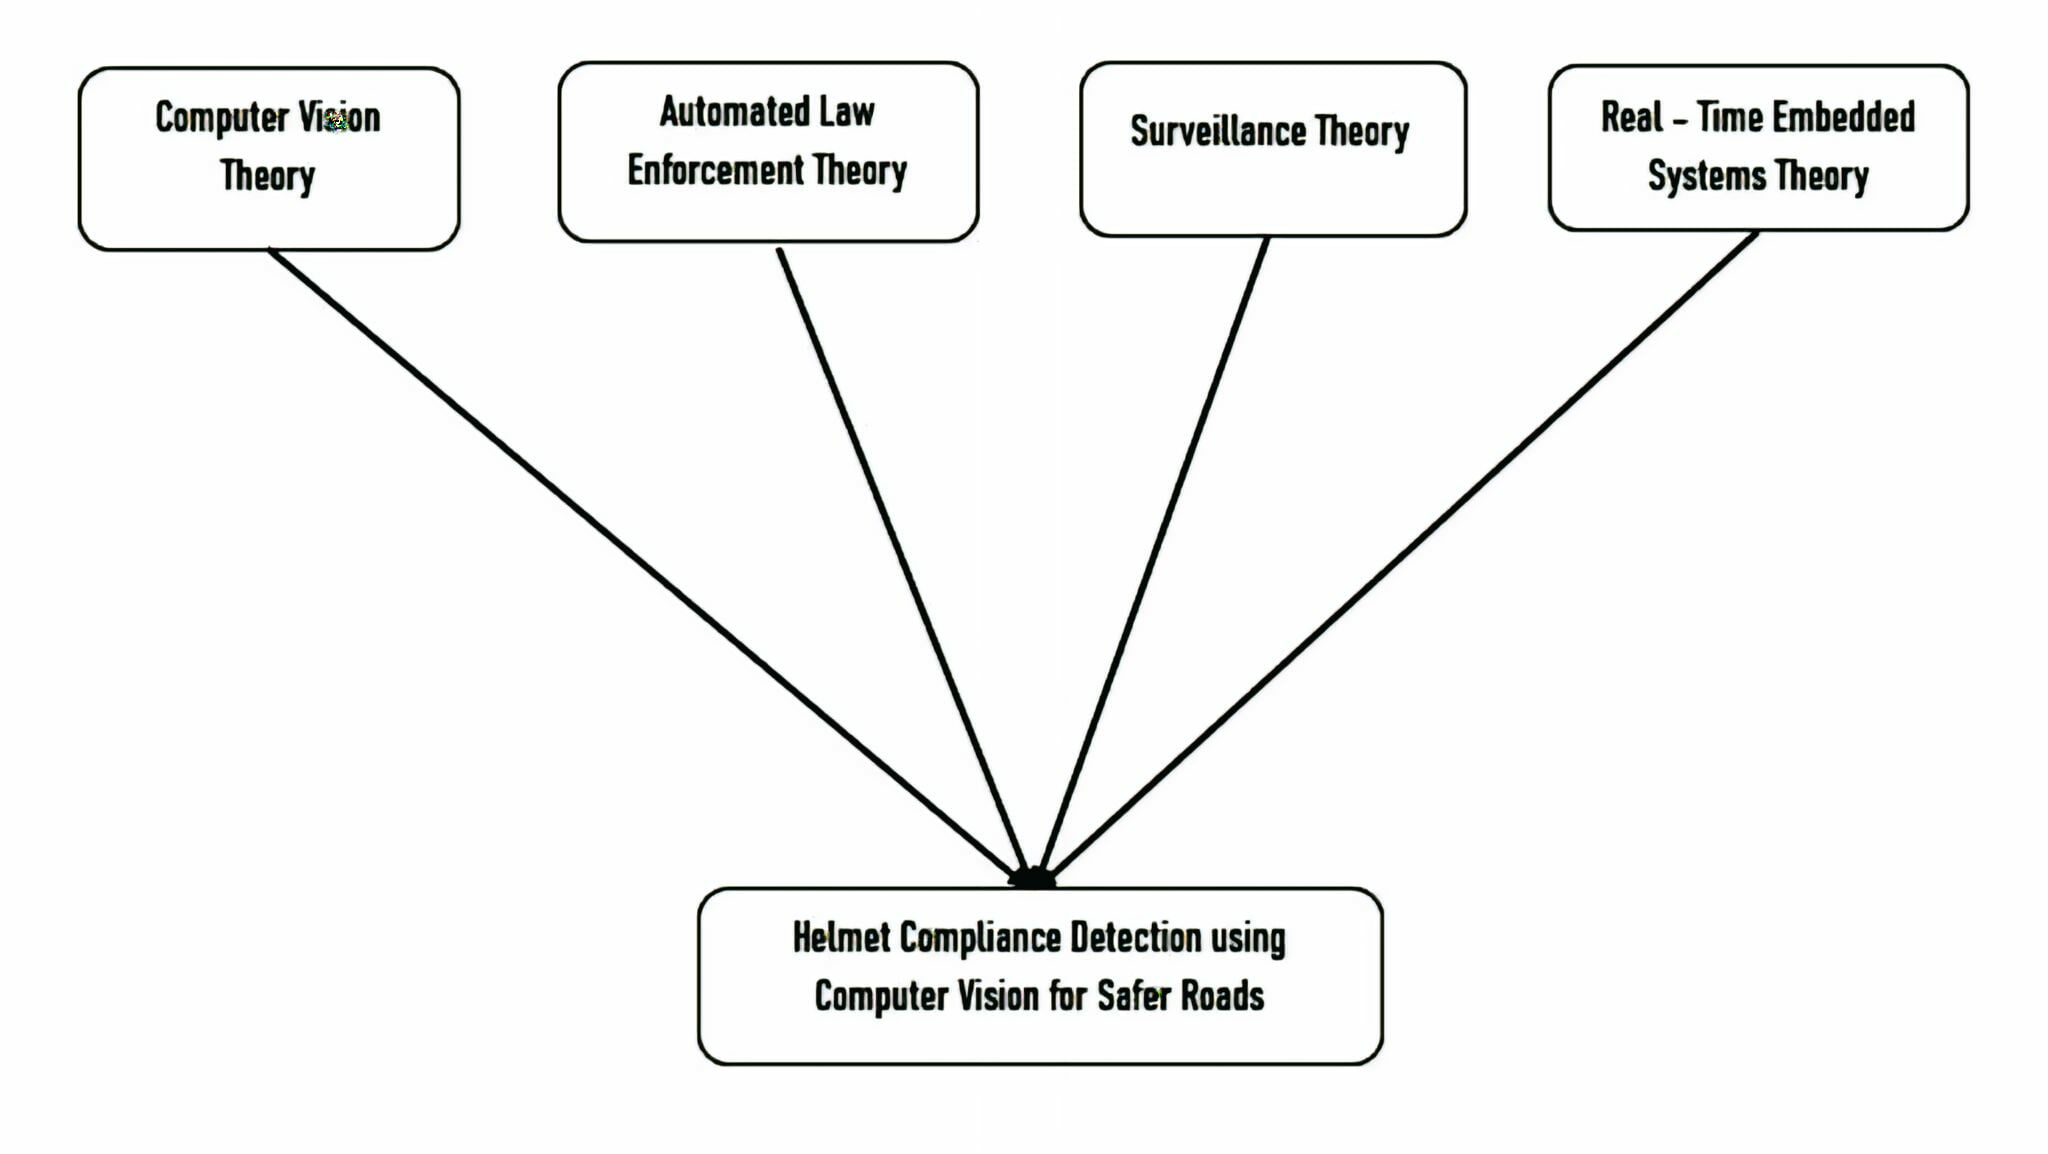
\includegraphics[width=0.9\textwidth]{figures/Fig 6.jpg}
    \caption{\textbf{Theoritical Framework of the Helmet Compliance Detection }}
    \label{figures/Fig 6.jpg}
\end{figure}
Figure 6 presents a simplified visual representation of the theoretical framework guiding the development of the Helmet Compliance Detection Prototype. The theoretical frame- work is supported by four foundational theories: Computer Vision Theory, Automated Law Enforcement Theory, Surveillance Theory, and Real-Time Embedded Systems The- ory. Each of these theories is directly connected to the framework, illustrating how they collectively inform and strengthen the system’s design and functionality. The layout em- phasizes the multidisciplinary nature of the project, integrating both technical and soci- ological perspectives to ensure operational efficiency, real-time performance, and social relevance.


\subsection{Computer Vision Theory}
This theory provides the foundation for interpreting and processing visual inputs (video or image data) to extract meaningful patterns. In this prototype, YOLOv8 is applied to enable real-time detection of motorcycles, riders’ helmet compliance, and overloading violations.



\subsection{Automated Law Enforcement Theory}
This theory emphasizes the role of intelligent systems in supporting or replacing human roles in enforcing regulations. In the context of traffic compliance, the integration of technologies such as OpenCV and YOLOv8 aligns with the principles of automation for more accurate, consistent, and scalable monitoring.


\subsection{Surveillance Theory}
Surveillance Theory explains the sociotechnical importance of systematically observing and recording behaviors to ensure safety and rule compliance. This theory justifies the deployment of camera-based monitoring systems in public spaces to detect and deter traffic violations, promoting accountability and public safety.


\subsection{Real-Time Embedded Systems Theory}
This theory supports the technical design of prototypes that process data and respond within strict time constraints. It underpins the implementation of real-time detection features in the system, enabling low-latency processing of live video feeds through optimized algorithms and embedded computing environments.




\
%=======================================================%
%%%%% Do not delete this part %%%%%%
\clearpage


\printbibliography[heading=subbibintoc, title={\texorpdfstring{\centering}{} Notes}]
\end{refsection}
